\section{项目开发与迭代优化}

\subsection{初始开发与实际安排}
项目初期先搭建可运行的客户端，用示例课表与本地数据检验页面组织和课程模型，再接入江财教务、学习通与校园生活服务。校方课表结构需要逐步验证，饮水登录也经过多次排查。开发因此调整了顺序，优先解决教务登录循环和缓存显示，并先在生活模块验证真实账户查询。随后完善独立待办和课程活跃度管理，并集中整理账号入口及各页交互。图\ref{fig:timeline}概括了主要阶段及其成果。

\begin{figure}[htbp]
\centering\begin{tikzpicture}
\node[block,text width=29mm,minimum height=21mm] (a) at (-6,0) {\textbf{初步设计}\\客户端与课表模型};
\node[block,text width=29mm,minimum height=21mm] (b) at (-2,0) {\textbf{教务接入}\\课表同步\\会话处理完善};
\node[block,text width=29mm,minimum height=21mm] (c) at (2,0) {\textbf{核心业务完善}\\待办、任务管理\\饮水服务查询};
\node[block,text width=29mm,minimum height=21mm] (d) at (6,0) {\textbf{使用流程整合}\\集中管理账号\\统一界面设计};
\foreach \first/\last in {a/b,b/c,c/d}{\draw[flow] (\first) -- (\last);}
\end{tikzpicture}

\caption{项目主要开发与迭代阶段}\label{fig:timeline}
\end{figure}

\subsection{教务接入与启动登录循环}
初期的模拟适配器和本地导入可以验证课程模型及离线展示，但更新课表仍需用户准备材料。实际检查发现，校方登录首页不足以定位课表，个人课表则包含星期、周次、节次及地点等可解析信息。酱菜通在用户认证后读取个人课表，以独立的校历映射处理校方学期选项，再将读取、校验与缓存更新串成自动同步流程。261 和 252 两个学期均取得真实课表，原有课程模型也继续用于展示同步结果。

接入后，模拟器上的冷启动曾反复弹出教务认证窗口。检查发现，会话已过期与启动后尚待核验共用一条路径，认证窗口关闭后，主界面恢复又满足原来的触发条件。为此，酱菜通将主动授权和静默读取分开，使用独立服务核验会话，并记下已确认的失效状态。实验中，用户主动重连后手动触发后台读取，更新时间随之推进，主界面保持可用。离线或会话失效时，应用仍显示原缓存。这次实验验证了后台读取路径，未等待六小时周期自行触发。

成绩查询也经历了从观察到调整的过程。校方默认选项曾返回空报表，我在校方页面核对了“有效成绩”的查询步骤。酱菜通随后从“入学以来”的报表识别有记录的学期，再按学期核验成绩。实验成功切换 252、251、242、241 四个学期，切回后确认缓存可用。这说明成绩页需要按校方可查结果组织学期，独立于课表能够展示的学期范围。

\subsection{学习通扫描及课程管理}
早期页面已能读取课程任务，但历史教学班与当前课程共同占用列表。按创建时间直接筛除旧教学班，会遗漏在旧课程中重新发布的内容。酱菜通以作业和通知的变化判断活跃度，分别保存可见状态和最近检查信息。统一后的扫描在同一轮读取分项任务，并检查到期的隐藏课程，课程列表和任务筛选共享查询结果。

一次真实扫描共处理 63 个教学班，其中 55 个完成全部分项读取，另有 8 个教学班的部分信息未完整返回。这个结果说明完整性需要按分项判断，成功读取的结果可以继续使用。实测也确认，隐藏课程仍可进入作业和活动复查。三十天阈值、新内容恢复以及旧标识重新出现时的处理通过合成输入检验

\subsection{798 协议适配和真实登录}
酱菜通早期发送短信验证码时取得业务码 0，登录请求却返回 $-1$。收到短信只确认了申请环节。酱菜通对照 life-798 的图形码标识、短信和登录请求、双账号通道与会话管理，定位了可逐项核查的协议边界。此后调整了图形码状态、会话保持及签名配置，并核对了旧版调用链，模拟器和真机仍出现登录失败。已有记录无法把拒绝归因于单一字段。

为进一步缩小排查范围，核对可用客户端的请求行为，并逐项核查请求头、序列化和原生会话行为，然后构建新的请求和页面处理代码，接入本机网络桥接与独立会话存储。完成短信验证后，登录返回业务码 0，随后读取了余额、收藏设备和消费账单，重启后仍可查询。

\subsection{页面布局和操作流程}
账号中心统一了授权入口后，课表页下方仍有重复登录卡和旧导入入口，“我的”也保留了一张独立介绍卡。项目移除这些容器，并继续允许从账号中心重连和回读已保存的课表。界面改进随后调整配色、标题层级、数据列表和弹层布局，让不同模块使用一致的视觉规则。图\ref{fig:beforeafter}展示同一测试账户、同一示例课表在 360 dp 视口下的效果。两张画面按相同范围裁切。修改前后均可选择学期和周次、切换周视图与日视图并刷新课表。

\begin{figure}[!htb]
\centering
\begin{tabular}{@{}c@{\hspace{5mm}}c@{}}
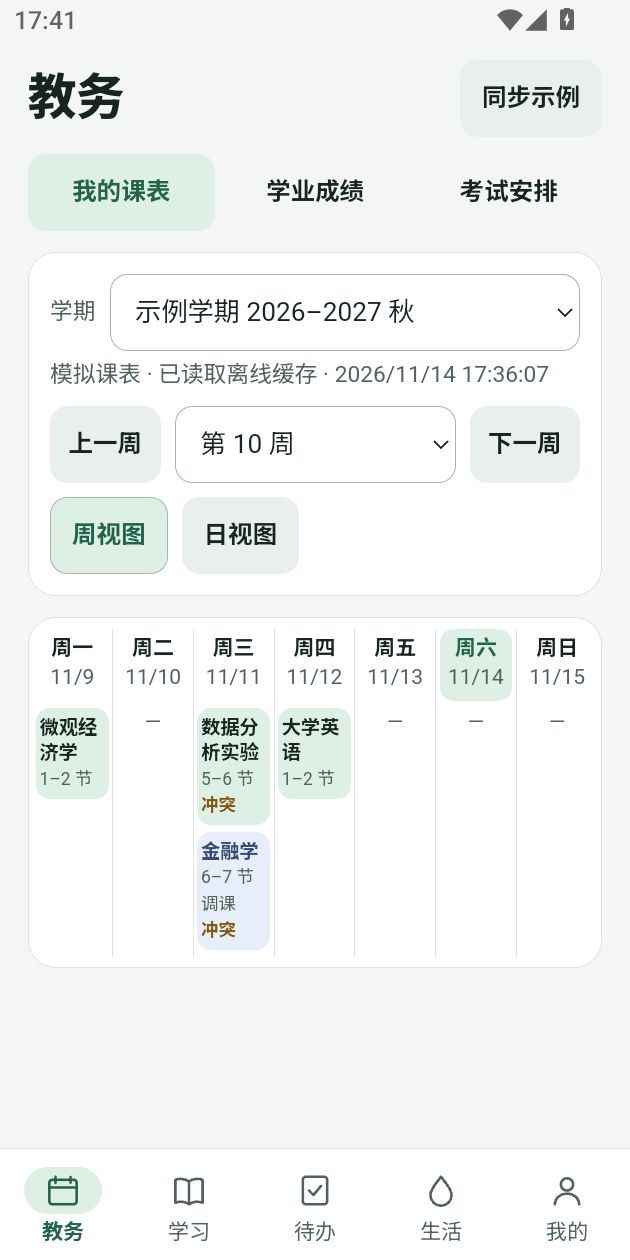
\includegraphics[width=.41\linewidth,trim=0bp 234bp 0bp 36bp,clip]{before-schedule.png} &
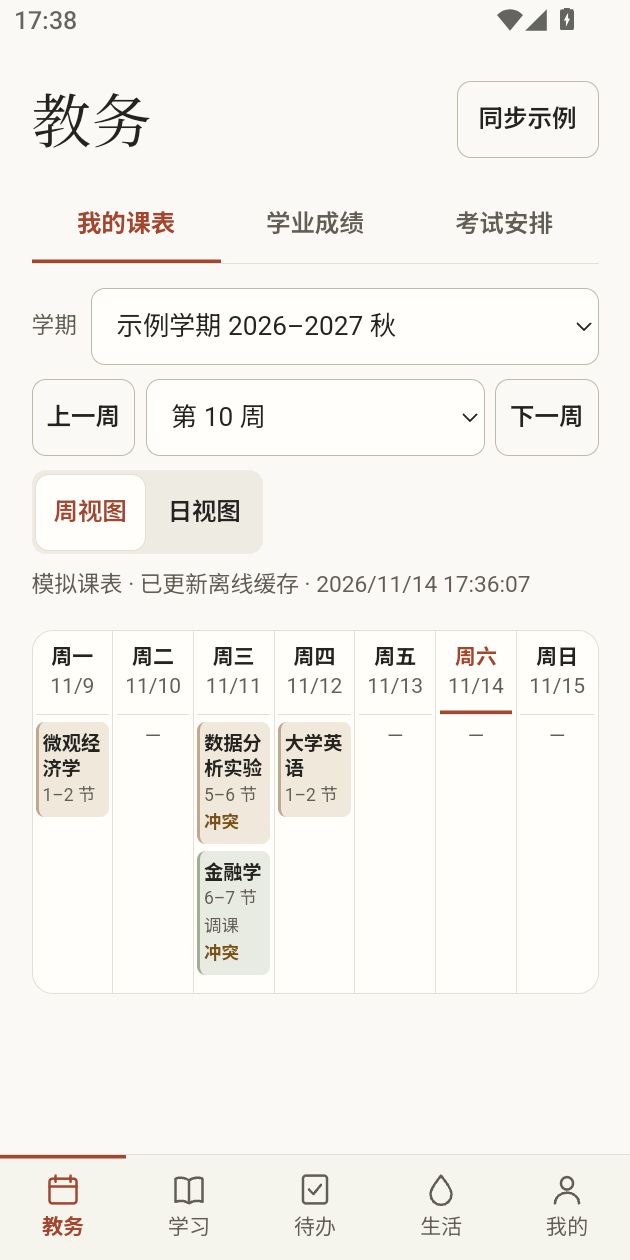
\includegraphics[width=.41\linewidth,trim=0bp 234bp 0bp 36bp,clip]{after-schedule.png} \\
\small 0.9.2 & \small 0.9.3 \\
\end{tabular}
\caption{同尺寸模拟器中的教务课表前后对比}\label{fig:beforeafter}
\end{figure}

\subsection{迭代效果分析}
表\ref{tab:changes}将发现的问题、改进措施和观察到的结果并列。由此可以看出，缓存显示、任务分项完整性与真实账户查询分别需要通过不同的操作验证。

\begin{table}[!htb]
\centering\small
\caption{代表性迭代的问题、措施及实际效果}\label{tab:changes}
\begin{tabularx}{\linewidth}{@{}>{\raggedright\arraybackslash}p{33mm}YY@{}}
\toprule
问题与证据 & 修改及其依据 & 验证结果 \\
\midrule
课表更新依赖手工准备材料 & 已授权页面能读到个人课表，遂以校方网格及校历驱动原有模型 & 两个学期读取成功，自动同步可替换同账号同学期旧结果 \\
会话失效后多次弹出认证 & Activity 恢复反复触发旧逻辑，分离交互认证与静默读取 & 主动重连后后台同步成功，离线和失效时保留课表 \\
历史课程影响当前任务查找 & 采用通知和作业判定活跃度，隐藏项仍纳入原扫描调度 & 实际扫描保留已读分项，隐藏项可继续复查，恢复规则通过合成测试 \\
798 短信成功后登录被拒 & 参考 life-798 分析流程，借可登录客户端确认请求与会话差异 & 本人登录后读取余额、设备与账单，重启后可以再次查询 \\
\bottomrule
\end{tabularx}
\end{table}
